\documentclass[9pt]{beamer}

\usepackage{amsmath,amssymb,amstext,amsfonts,setspace,dsfont,amsmath,amsthm,array,nomencl,hyperref,pgf,xcolor}

\usepackage{beamerthemesplit}

%\usetheme{Dresden}
\usetheme{Ilmenau}

\setbeamertemplate{navigation symbols}{} %no navigation symbols

\setbeamertemplate{footline}
{%
\leavevmode%
\hbox{%

\begin{beamercolorbox}[wd=.3\paperwidth,ht=2.5ex,dp=1.125ex,left]{author
in head/foot}%
\usebeamerfont{author in head/foot}\hspace{.3cm}\insertshortauthor\hspace{.3cm}
\end{beamercolorbox}%

\begin{beamercolorbox}[wd=.5\paperwidth,ht=2.5ex,dp=1.125ex,center]{title
in head/foot}%
\usebeamerfont{title in head/foot}\hspace{.3cm}\insertshorttitle
\end{beamercolorbox}%

\begin{beamercolorbox}[wd=.2\paperwidth,ht=2.5ex,dp=1.125ex,right]{author
in head/foot}%
\usebeamerfont{author in head/foot}Slide\hspace{.1cm}\insertframenumber\hspace{.1cm}of\hspace{.1cm}\inserttotalframenumber\hspace{.3cm}
\end{beamercolorbox}%
}%
\vskip0pt%
}

\setbeamertemplate{blocks}[rounded][shadow=true]

\title{Linear and Differential Cryptanalysis of DES}
\author{Slava Chernyak and Sourav Sen Gupta}
\institute{University of Washington}
\date{February 2, 2009}

\begin{document}

\begin{frame}
\titlepage
\end{frame}

\section{Introduction}

\begin{frame}
\begin{beamercolorbox}[ht=2.5ex,dp=1.125ex,center,rounded=true,shadow=true]{author in head/foot}
A quick review of DES
\end{beamercolorbox}
\end{frame}

\subsection{Data Encrytption Standard}
\begin{frame}
\begin{columns}
\begin{column}{0.6\textwidth}
\begin{block}{DES Function}
\[ DES : (\mbox{Plaintext }(P), \mbox{ Key }(K))  \mapsto \mbox{Cipher }(C) \]
\end{block}

\begin{block}{DES Unit Blocks}
\begin{align*}
\sigma_{i+1} : \: & (0,1)^{64} \rightarrow (0,1)^{64} \\
& (L_i, R_i) \mapsto (L_i \oplus f(R_i,K_{i+1}), R_i) \\
\tau : \: & (0,1)^{64} \rightarrow (0,1)^{64} \\
& (L_{i+1},R_{i+1}) \mapsto (R_{i+1},L_{i+1})
\end{align*}
\end{block}

\begin{itemize}
\item{Input for round $i+1$: $(L_i,R_i)$}
\item{Subkey for round $i+1$: $K_{i+1}$}
\item{Feistel function ($f$)}
\item{16-rounds for $i = 0, 1, ..., 15$}
\end{itemize}

\end{column}
\begin{column}{0.4\textwidth}
\begin{figure}
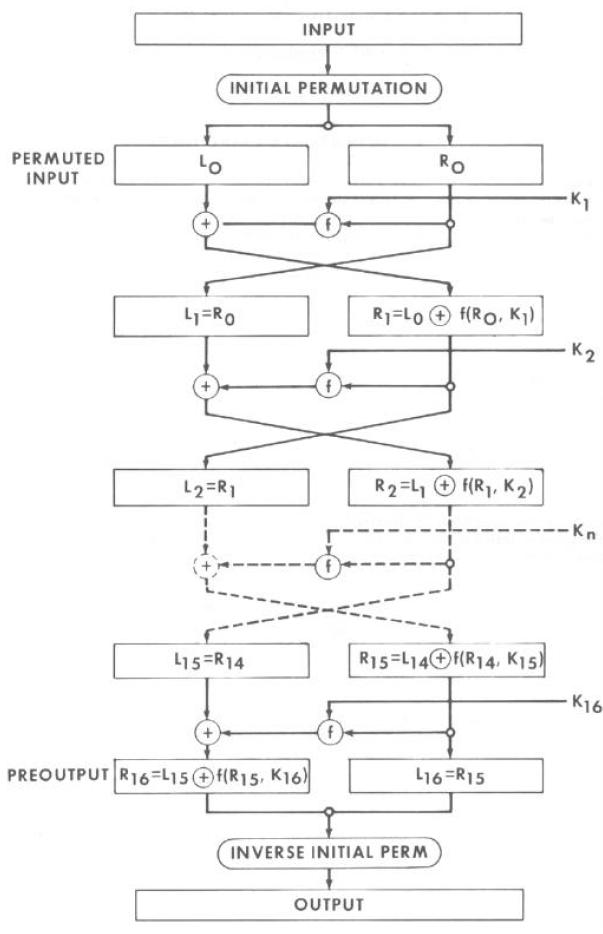
\includegraphics[totalheight=0.8\textheight]{des_algo.jpg}
\caption{DES Algorithm}
\end{figure}
\end{column}
\end{columns}
\end{frame}

\begin{frame}
\begin{columns}
\begin{column}{0.45\textwidth}
\begin{block}{Feistel Function}
\begin{align*}
f : \: & (0,1)^{32} \times (0,1)^{48} \rightarrow (0,1)^{32} \\
& (R,K)  \mapsto P (S_{Box}(E(R) \oplus K)) 
\end{align*}
\end{block}

\begin{itemize}
\item{Right half of the plaintext ($R$)}
\item{Expansion function \\ $E : (0,1)^{32} \rightarrow (0,1)^{48}$}
\item{Key for the round ($K$)}
\item{Confusion function (S-Boxes) \\ $S_i: (0,1)^6 \rightarrow (0,1)^4$}
\item{Diffusion function \\ $P : (0,1)^{32} \rightarrow (0,1)^{32}$}
\end{itemize}
\end{column}
\begin{column}{0.55\textwidth}
\begin{figure}
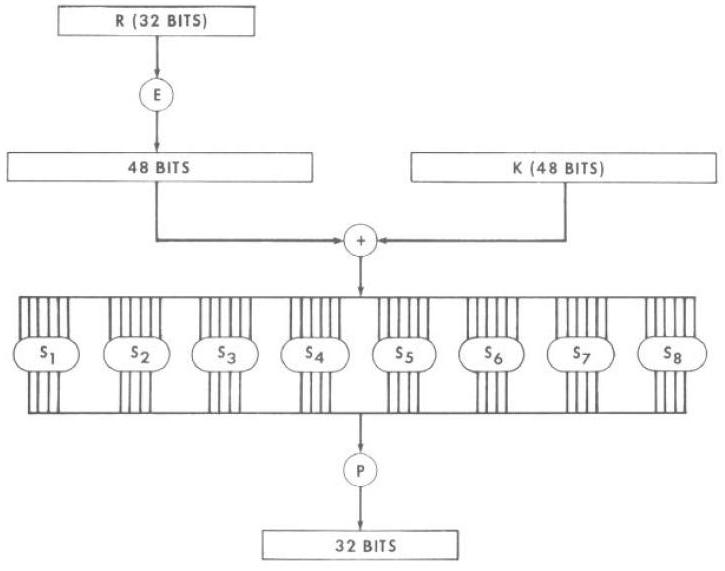
\includegraphics[totalheight=0.6\textheight]{des_feistel.jpg}
\caption{Feistel Round for DES}
\end{figure}
\end{column}
\end{columns}
\end{frame}

\begin{frame}
Mathematically, the different pieces of DES are:
\begin{itemize}
\item{Initial Permutation $IP : (0,1)^{64} \rightarrow (0,1)^{64}$}
\item{DES Unit Block functions $\sigma_{i+1} (L_i,R_i)$ for $i = 0,1,...,15$}
\item{Transpositions $\tau : (L_{i+1},R_{i+1}) \mapsto (R_{i+1},L_{i+1})$ for $i = 0,1,...,14$}
\item{Inverse Initial Permutation $IP^{-1} : (0,1)^{64} \rightarrow (0,1)^{64}$}
\end{itemize}

\begin{block}{Algebraic Representation of DES}
\begin{align*}
C &= DES_K (P) = IP^{-1} \sigma_{16} \tau \cdots \tau \sigma_1 IP (P) \\
P &= DES^{-1}_K (C) = IP^{-1} \sigma_{1} \tau \cdots \tau \sigma_{16} IP (C)
\end{align*}
\end{block}

Note: The inverse DES comes from the fact that $\tau^2 = \sigma_i^2 = 1$
\end{frame}

\subsection{Linear Cryptanalysis}
\begin{frame}
\begin{beamercolorbox}[ht=2.5ex,dp=1.125ex,center,rounded=true,shadow=true]{author in head/foot}
Basic Idea of Linear Cryptanalysis
\end{beamercolorbox}
\end{frame}

\begin{frame}
Linear Attack on DES idea:\\
\begin{itemize}
\item S-Boxes depend on a relatively small number of bits (6) which allows us to write down linear (or afine) expressions that approximate S-Boxes \\
\item The effects of one round do not diffuse quickly over following rounds. Thus linear expresions (as above) that hold per-round can be combined across rounds.
\end{itemize}
\end{frame}

\begin{frame}
Specifically, if $P_{i}$ are plaintext bits, $C_{i}$ are cyphertext bits, and $K_{i}$ are subkey bits, then we wish to find an expression of the form
\[ P_{i_1} \oplus P_{i_2} \cdots P_{i_j} \oplus C_{i_1} \oplus C_{i_2} \cdots C_{i_k} = K_{i_1} \oplus K_{i_2} \oplus K_{i_m} \]
Such that this expression has a high \textit{or} low probability of occurence.\\
\vspace{5mm}
Consider: No such obvious expression should exist, otherwise the cipher is trivially weak. If we were to randomly select bits for the above expression, it would hold exactly $1/2$ the time. If we find an expression such as above that displays a high \textit{bias}, that is, it holds much more or less freqently than $1/2$ the time, we can exploit this.
\end{frame}


\subsection{Differential Cryptanalysis}
\begin{frame}
\begin{beamercolorbox}[ht=2.5ex,dp=1.125ex,center,rounded=true,shadow=true]{author in head/foot}
Basic Idea of Differential Cryptanalysis
\end{beamercolorbox}
\end{frame}

\begin{frame}
\begin{definition}[Differential]
Suppose two plaintext inputs to the system be $X$ and $X'$ with corresponding output ciphertexts $Y$ and $Y'$ respectively. Then the pair of input difference ($\Delta X = X \oplus X'$) and the output difference ($\Delta Y = Y \oplus Y'$) is called a {\it differential} for the system.
\end{definition}

Vulnerability of DES:\\
Differential Cryptanalysis exploits the high probability of certain occurrences of differential patterns in the cipher. In DES, this highly probable differentials occur due to
\begin{itemize}
\item{S-Boxes show a strong tendency to produce certain differential pairs with high probability, rather than being random.}
\item{The differences do not get diffused fast enough.}
\item{Differentials are not affected by the round keys.}
\end{itemize}
\end{frame}

\begin{frame}
In an $k$-round DES, we can trace the path of a certain input difference to get an output difference with a high probability. This tracing path is known as a {\it differential characteristic}.

\[ \Delta P \rightarrow \Delta X_1 \rightarrow \Delta X_2 \rightarrow \cdots \rightarrow \Delta X_{k-1} \rightarrow \Delta C \]

In an ideal situation, one will expect the probability
\[ P \left(\Delta C | \Delta P \right) = \frac{1}{2^n} \]
for an $n$-bit cipher system. Differential attacks seek to exploit a scenario where
\[ P \left(\Delta C | \Delta P \right) = p_D \gg \frac{1}{2^n} \]

This is essentially a chosen-plaintext attack as we want the specific input difference to occur for every pair.
\end{frame}

\section{Mathematical Framework}
\begin{frame}
\begin{beamercolorbox}[ht=2.5ex,dp=1.125ex,center,rounded=true,shadow=true]{author in head/foot}
Dive into the Mathematics
\end{beamercolorbox}
\end{frame}

\subsection{Substitution-Permutation Network}

\begin{frame}
\begin{columns}
\begin{column}{0.6\textwidth}
\begin{figure}
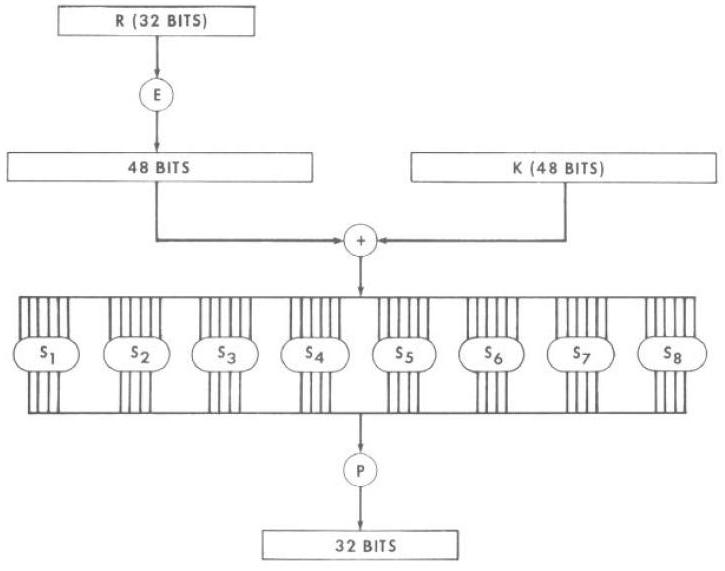
\includegraphics[totalheight=0.5\textheight]{des_feistel.jpg}
\end{figure}
Let us simplify DES by
\begin{itemize}
\item{Reducing the bitlength from $64$ to $16$}
\item{Removing expansion function $E(R)$}
\item{Taking identical S-Boxes of size $4$ bits}
\item{Repeating over less rounds}
\end{itemize}
\end{column}

\begin{column}{0.4\textwidth}
\begin{figure}
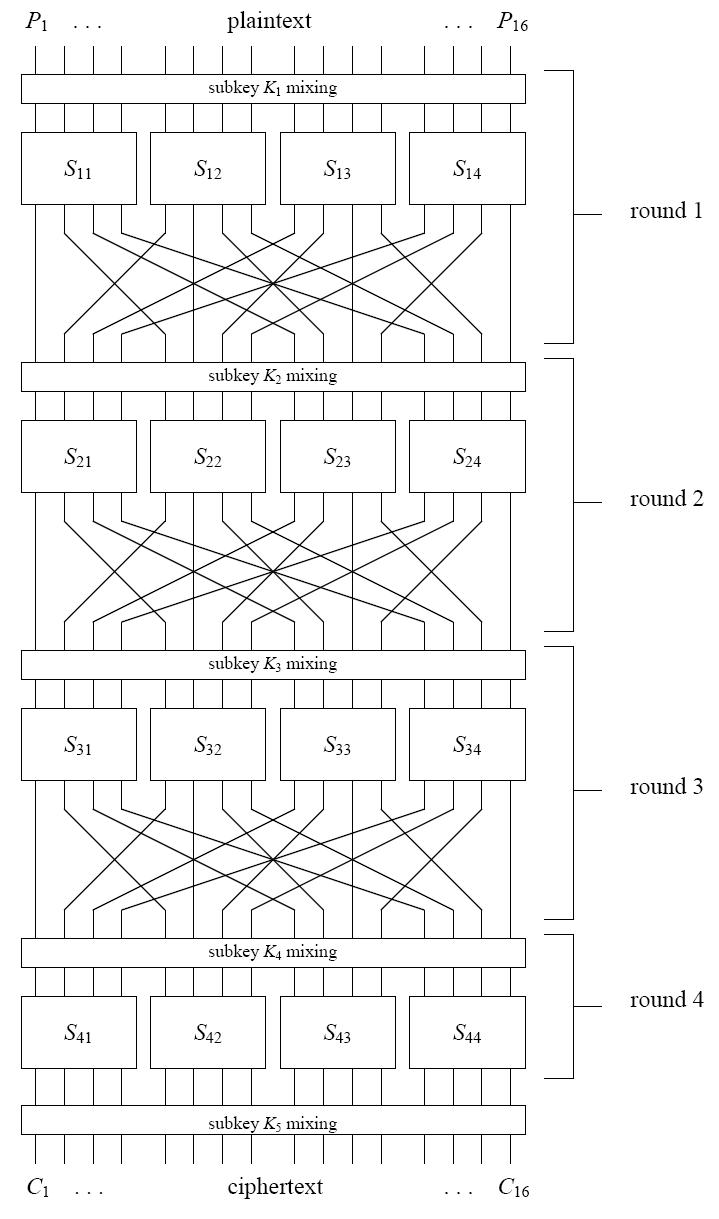
\includegraphics[totalheight=0.8\textheight]{spn.jpg}
\end{figure}
\end{column}
\end{columns}

\begin{center}
{\tiny Disclaimer: This simplification does not affect the discussion of the techniques of Linear/Differential Cryptanalysis.}
\end{center}
\end{frame}

\begin{frame}
\begin{beamercolorbox}[ht=2.5ex,dp=1.125ex,center,rounded=true,shadow=true]{author in head/foot}
Simple Substitution-Permutation Network
\end{beamercolorbox}
\end{frame}

\begin{frame}
We define a simple Substitution-Permutation Network Cipher (SPN) which has structural similarity to DES.

\begin{itemize}
\item SPN is a 16-bit block cipher (16-bit plaintext to 16-bit ciphertext) with 16-bit round keys.
\item Each round consists of a substitution and a permutation (much like in DES)
\item The substitution is the result of splitting the 16-bit input block to a round in to 4 4-bit sub-blocks. Each 4-bit sub-block is then mapped across a 4-bit to 4-bit S-box. We use the same S-box throughout.
\item The permutation is applied to all 16-bits of the round following the substitution.
\item Finally, key-mixing is achieved by XOR-ing the round key with every input block to a round as well as at the end of the last round (so that we can't simply ignore the last round)
\item The SPN cipher we will look at will consist of 4 rounds.
\end{itemize}
\end{frame}

\begin{frame}
SPN S-Box and Permutation:\\
\vspace{5mm}
SPN uses a single 4-bit S-Box that has the following structure:
\begin{figure}
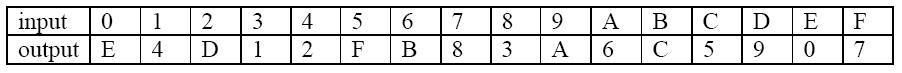
\includegraphics[width=0.9\textwidth]{spn_sbox.jpg}
\end{figure}

\vspace{5mm}
And the following 16-bit permutation:
\begin{figure}
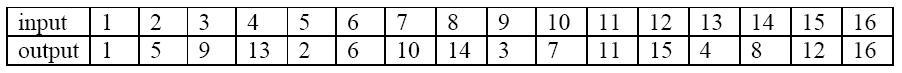
\includegraphics[width=0.9\textwidth]{spn_perm.jpg}
\end{figure}

\vspace{5mm}

\end{frame}

\subsection{Linear Attack on SPN}
\begin{frame}
\begin{beamercolorbox}[ht=2.5ex,dp=1.125ex,center,rounded=true,shadow=true]{author in head/foot}
Mathematics of Linear Cryptanalysis
\end{beamercolorbox}
\end{frame}

\begin{frame}
\large{Basic Definitions for the Linear attack:}\\
\vspace{5 mm}
Linear cryptanalysis tries to take advantage of high probability occurrences of linear expressions involving plaintext bits, ciphertext bits and subkey bits. It is a known plaintext attack.\\
\vspace{5 mm}
Define $P_i$ where $i = 1, 2, \dots 16$ as the $i$-th plaintext bit.\\
Define $C_i$ where $i = 1, 2, \dots 16$ as the $i$-th cyphertext bit.\\
Define $U_{j,i}$ where $j = 1, 2, 3, 4$ and $i = 1, 2, \dots 16$ be the $i$-th input bit to the $j$-th round of SPN.\\
Define $V_{j,i}$ where $j = 1, 2, 3, 4$ and $i = 1, 2, \dots 16$ be the $i$-th output bit of the $j$-th round of SPN.\\
\end{frame}

\begin{frame}
Linear and Affine approximation of S-Box:\\
\vspace{5mm}
How do we come up with the desired expression for the entire cipher? We start by looking at the only non-linear component, the S-Box.\\
\vspace{5mm}
To find the linear/afine approximation of the S-Box we simply consider every possible expression of the input bits $X_i$ and output bits $Y_j$. Thus the expression has the form
\[ \bigoplus_{i \in U} X_i = \bigoplus_{j \in V} Y_j \]
Where $U$ and $V$ range over all possible subsets of $\{1, 2, 3 ,4\}$. We then compare how often this expression coincides with the S-Box. \\
\vspace{5mm}
Note that there are 16 possibilities for $U$ and $V$, hence 256 total possible expressions. (this is for a 4-bit S-box)
\end{frame}

\begin{frame}
S-Box approximatin example:\\
\vspace{5mm}
We can take the following expression as an example:
\[ X_2 \oplus X_3 = Y_1 \oplus Y_3 \oplus Y_4 \]
Applying all possible values for the input $X$ bits it turns out that the expression holds in 12 out of the 16 cases. Hence, this expression has a bias of $12/16 - 1/2 = 1/4$.\\
\vspace{5mm}
Similarly the following expression
\[ X_3 \oplus X_4 = Y_1 \oplus Y_4 \]
Has a bias of $-3/8$, which is higher in magnitude than the previous one. It is the magnitude of the bias that is important.
\end{frame}

\begin{frame}
The number of agreements (minus 8) between the S-Box and every possible expression is summarized in the table below. Thus to get the bias, one must only divide by 16.\\
\vspace{5mm}
\begin{figure}
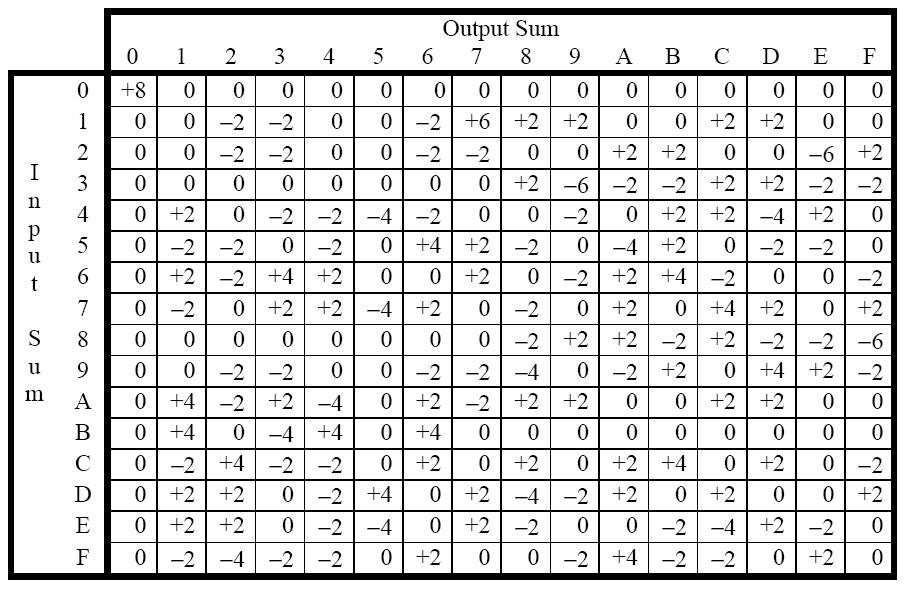
\includegraphics[height=0.7\textheight]{spn_linear_approx.jpg}
\end{figure}
\end{frame}


\begin{frame}
What this means for 1 Round:\\
\vspace{5mm}
Note, from the previous table, that the expression $X_1 \oplus X_3 \oplus X_4 = Y_2$ has a bias of $+1/4$. \\
\vspace{5mm}
Note also that $U_1 = P \oplus K_1$. 
\vspace{5mm} We can now write down the following linear approximation across the 1st round of SPN:
\begin{eqnarray*}
V_{1,6} & = & U_{1,5} \oplus U_{1,7} \oplus U_{1,8} \mbox{  $\leftarrow$ S-Box approximation above}\\
		  & = & (P_5\oplus K_{1,5}) \oplus (P_7\oplus K_{1,7}) \oplus (P_8\oplus K_{1,8})
\end{eqnarray*}
This expression holds with probability of $3/4$ (bias of $+1/4$)
\end{frame}

\begin{frame}
We can get expressions that hold with some non-$1/2$ probability for every round. But we must somehow combine them to write an expression relating the plaintext and ciphertext bits $\Rightarrow$ We use the Piling Up Principle:\\
\vspace{5mm}
Note: \\
$X_1 \oplus X_2 = 0$ is a linear expression equivalent to $X_1 = X_2$\\
$X_1 \oplus X_2 = 1$ is an affine expression equivalent to $X_1 \neq X_2$\\
\vspace{5mm}
Assume the following probability distribution
\[ Pr(X_1 = i)  = \left\{ \begin{array}{ll}
         p_1 & \mbox{$i = 0$};\\
         (1 - p_1) & \mbox{$i = 1$}.\end{array} \right. \] 
\[ Pr(X_2 = i)  = \left\{ \begin{array}{ll}
         p_2 & \mbox{$i = 0$};\\
         (1 - p_2) & \mbox{$i = 1$}.\end{array} \right. \] 
\end{frame}

\begin{frame}
Piling Up Principle Continued:\\
\vspace{5mm}
Assuming that $X_1$ and $X_2$ are independant:
\[ Pr(X_1 = i, X_2 = j)  = \left\{ \begin{array}{ll}
         p_1 p_2 & \mbox{$i = 0, j = 0$};\\
         (1 - p_1) p_2 & \mbox{$i = 1, j = 0$} \\
			p_1 (1 - p_2) & \mbox{$i = 0, j = 1$} \\
			(1 - p_1)(1 - p_2) & \mbox{$i = 1, j = 1$}.\end{array} \right. \] 
Now, note that $X_1 \oplus X_2 = 0 \Rightarrow X_1 = 1, X_2 =1$ OR $X_1 = 0, X_2 = 0$. Hence:
\begin{eqnarray*}
 Pr(X_1 \oplus X_2 = 0) & = & Pr(X_1=0,X_2=0) + Pr(X_1=1,X_2=1) \\
								& = & p_1p_2 + (1 - p_1)(1-p_2)
\end{eqnarray*}
If we write $p_k = 1/2 + \epsilon_k$ we have
\[ Pr(X_1 \oplus X_2 = 0) = 1/2 + 2\epsilon_1 \epsilon_2 \]
Hence the bias of $X_1 \oplus X_2 = 0$ is 
\[ 2 \epsilon_1 \epsilon_2 \]
That is, twice the product of the bias of the original expressions.
\end{frame}

\begin{frame}
Piling Up Principle Continued - The Piling Up Lemma:\\
\vspace{5mm}
We extend the idea on the previous slide to the general case: For $n$ independant random binary variables, $X_1, X_2, \dots, X_n$, 
\[ Pr(X_1 \oplus X_2 \cdots \oplus X_n = 0) = 1/2 + 2^{n-1} \prod_{i=1}^n \epsilon_i \]
In terms of bias,
\[ \epsilon_{1,2,\dots,n} = 2^{n-1} \prod_{i = 1}^n \epsilon_i \]
Where $\epsilon_{1,2,\dots,n}$ is the total bias of $X_1 \oplus X_2 \cdots \oplus X_n = 0$. \\
\vspace{5mm}
Note that if some $\epsilon_k = 0$ (that is, some $X_k$ has no bias) then the total bias will be $0$.  
\end{frame}

\begin{frame}
Now, come back to Per-round approximations. We can write down 4 approximations (Let $S_{i,j}$ repesent the $j$-th S-Box in the $i$-th round):
\begin{eqnarray*}
S_{1,2}: X_1 \oplus X_3 \oplus X_4 & = & Y_2 \\
S_{2,2}: X_2 = Y_2 \oplus Y_4 \\
S_{3,2}: X_2 = Y_2 \oplus Y_4 \\
S_{3,4}: X_2 = Y_2 \oplus Y_4 \\
\end{eqnarray*}
Each of these has a probability bias magnitude of $1/4$. We can use the Piling Up Principle to combine them into a single expression relating plaintext bits to cyphertext bits.
\end{frame}

\begin{frame}
Consider the first 2 rounds:\\
\vspace{5mm}
\[  X_1 \oplus X_3 \oplus X_4 = Y_2 \Rightarrow \]
\[ V_{1,6} = (P_5\oplus K_{1,5}) \oplus (P_7\oplus K_{1,7}) \oplus (P_8\oplus K_{1,8}) \]
\vspace{2mm}
\[ X_2 = Y_2 \oplus Y_4 \Rightarrow \]
\[ V_{2,6} \oplus V_{2,8} = V_{1,6} \oplus K_{2,6} \]
\vspace{2mm}
Each of these has a bias of magnitude $1/4$. We can combine:
\[  V_{2,6} \oplus V_{2,8} \oplus P_5 \oplus P_7 \oplus P_8 \oplus K_{1,5} \oplus K_{1,7} \oplus K_{1,8} \oplus K_{2,6} = 0 \]
By the Piling Up Principle this expression holds with bias:
\[ 2 * 1/4 * 1/4 = 1/8 \]
Note the implicit assumption that S-Boxes are independant. More on this later.
\end{frame}

\begin{frame}
Using this principle we can write the following equation over 3 rounds of SPN:
\[ U_{4,6} \oplus U_{4,8} \oplus U_{4,14} \oplus U_{4, 16} \oplus P_5 \oplus P_7 \oplus P_8 = \Sigma K \]
Where $\Sigma K$ is the sum over some key bits. Note that Since the key is fixed, $\Sigma K = 0$ or $1$ and thus we can ignore it since we only care about the bias.\\
\vspace{5mm}
The magnitude of the bias of the above expression, by the Piling Up Principle, is $1/32$. \\
\vspace{5mm}
Next we show how we can extract key bits using this information.
\end{frame}

\begin{frame}
Attack Idea:\\
\vspace{3mm}
We have an expression that links plaintext bits to input bits to the 4th round of SPN that holds with high bias ($1/32$). We can partially undo the last round by guessing the last key. \\
\vspace{3mm}
\pause
If we guess correctly, the equation will hold with high bias. If we guess wrong, the equation will probabily hold with probability close to 1/2, that is, a bias close to 0.\\
\vspace{3mm}
\pause
BUT To do this, we don't need to guess the entire key for the last round! Our expression only involves 4 key bits, output from 2 S-Boxes. Thus we only need to guess $2^8 = 256$ values.\\
\vspace{3mm}
\pause
For each value of the guessed \textit{target partial subkey} we can undo the last round and determine the bias of the equation. Highest bias indicates likely correct guess.
\end{frame}

\begin{frame}
\begin{columns}
\begin{column}{0.45\textwidth}
\begin{block}{SPN Linear Approximation}
\begin{align*}
 U_{4,6} & \oplus U_{4,8} \oplus U_{4,14} \oplus U_{4, 16} \\
         & \oplus P_5 \oplus P_7 \oplus P_8 = 0 
\end{align*}
\end{block}
\end{column}
\begin{column}{0.55\textwidth}
\begin{figure}
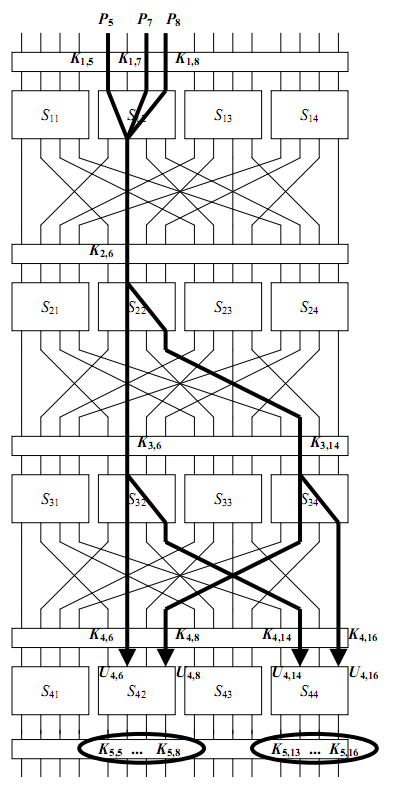
\includegraphics[totalheight=0.85\textheight]{SPN_linear.PNG}
\caption{Linear Attack on SPN}
\end{figure}
\end{column}
\end{columns}
\end{frame}

\begin{frame}
Probabalistic Justification:\\
\vspace{5mm}
In general, the number of plaintext-ciphertext pairs needed is related inversely-quadratically to the bias. That is
\[ N_{pairs} \approx 1 / \epsilon^2 \]
For the SPN cipher approximation with bias $1/32$ we need about $1000$ pairs. To perform the attack with near full probability of success.
\end{frame}

\subsection{Differential Attack on SPN}
\begin{frame}
\begin{beamercolorbox}[ht=2.5ex,dp=1.125ex,center,rounded=true,shadow=true]{author in head/foot}
Mathematics of Differential Cryptanalysis
\end{beamercolorbox}
\end{frame}

\begin{frame}
Basic math concepts behind Differential attack ...

\end{frame}

\begin{frame}
Intro to differentials ...

\end{frame}

\begin{frame}
Differential characteristic / approximation of SBox ...

\end{frame}

\begin{frame}
Probabilities for the approximations ...

\end{frame}

\begin{frame}
Analogue of Piling Up lemma ...

\end{frame}

\begin{frame}
Combining across SPN rounds ...

\end{frame}

\begin{frame}
The algorithm for the attack ...

\end{frame}

\begin{frame}
Probabilistic justification ...

\end{frame}

\subsection{Actual Attacks}
\begin{frame}
\begin{beamercolorbox}[ht=2.5ex,dp=1.125ex,center,rounded=true,shadow=true]{author in head/foot}
Let's get our hands dirty!
\end{beamercolorbox}
\end{frame}

\begin{frame}
Demo of attacks on SPN ... Runtime comparisons with Brute Force ...

\end{frame}

\begin{frame}
\begin{beamercolorbox}[ht=2.5ex,dp=1.125ex,center,rounded=true,shadow=true]{author in head/foot}
It's time for a Break!
\end{beamercolorbox}
\end{frame}


\section{Attacks on DES}
\begin{frame}
\begin{beamercolorbox}[ht=2.5ex,dp=1.125ex,center,rounded=true,shadow=true]{author in head/foot}
Do these work for DES?
\end{beamercolorbox}
\end{frame}

\subsection{Linear Attack: 3-round DES}
\begin{frame}
Linear Attack idea ...

\end{frame}

\begin{frame}
Matsui NS for SBoxes ...

\end{frame}

\begin{frame}
Linear approximations for SBoxes ...

\end{frame}

\begin{frame}
Piling up over 3 rounds ...

\end{frame}

\begin{frame}
Demo of the attack ...

\end{frame}

\subsection{Differential Attack: 3-round DES}
\begin{frame}
Differential Attack idea ...

\end{frame}

\begin{frame}
Differentials for SBoxes ...

\end{frame}

\begin{frame}
Differential characteristics for SBoxes ...

\end{frame}

\begin{frame}
Piling up over 3 rounds ...

\end{frame}

\begin{frame}
Demo of the attack ...

\end{frame}

\subsection{Extension to full DES}
\begin{frame}
Extension of the same ideas to 6 / 8 / 16 round DES ... Probabilistic explanation ...

\end{frame}


\section{Conclusion}
\begin{frame}
\begin{beamercolorbox}[ht=2.5ex,dp=1.125ex,center,rounded=true,shadow=true]{author in head/foot}
Did we miss anything important?
\end{beamercolorbox}
\end{frame}

\subsection{Independence of S-Boxes}
\begin{frame}
Refresh math idea ... Independence assumption ...

\end{frame}

\begin{frame}
What if that is false ? ... Discussion ...

\end{frame}

\subsection{Number of Pairs Required}
\begin{frame}
Probabilistic possibility of the attacks ... Pairs of data points needed ...

\end{frame}

\begin{frame}
Generalized attack idea on any given system ... Discussion ...

\end{frame}

\subsection{Links between the Attacks}
\begin{frame}
Links between Linear and Differential Attacks ...

\end{frame}

\begin{frame}
Mathematically and while implementing ...

\end{frame}

\subsection{Take Home}
\begin{frame}
\begin{beamercolorbox}[ht=2.5ex,dp=1.125ex,center,rounded=true,shadow=true]{author in head/foot}
`Take Home'
\end{beamercolorbox}
\end{frame}

\begin{frame}
If you are mounting the attacks ... To Do / Not To Do ...

\end{frame}

\begin{frame}
If you are building a cryptosystem ... To Do / Not To Do ...

\end{frame}

\begin{frame}
Questions ... Doubts ... Coding ... Misc ... Discussion ...

\end{frame}


\end{document}
